\documentclass[reprint, amsmath, amssymb, aps, prl]{revtex4-2}

\usepackage{graphicx}
\usepackage{dcolumn}
\usepackage{bm}
\usepackage{booktabs}
\usepackage{hyperref}
\usepackage{algorithm}
\usepackage{algpseudocode}

\hypersetup{
    colorlinks=true,
    linkcolor=blue,
    filecolor=magenta,      
    urlcolor=cyan,
}

\begin{document}

\pagestyle{plain}

\preprint{APS/123-QED}

\title{Four New Hybrid Root Bracketing Algorithms: Optimization-Based Approaches for Numerical Root Finding}

\author{Abdelrahman Ellithy}
\email{abdelrhmanellithy@gmail.com}
\affiliation{Department of Scienc, Faculty of Computers and Artificial Intelligence, Benha University, Benha, Egypt}

\author{Ahmed Shalaby}
\affiliation{Department of Computer Science, Faculty of Computers and Artificial Intelligence, Benha University, Benha, Egypt}

\author{Elsayed Badr}
\affiliation{Department of scientific Computing, Faculty of Computers and Artificial Intelligence, Benha University, Benha, Egypt}

\date{\today}

\begin{abstract}
This paper presents four novel hybrid root bracketing algorithms that combine the advantages of traditional bracketing methods with optimization techniques. The proposed algorithms—Optimized Bisection-False Position (Optimized\_BF), Optimized Bisection-False Position with Modified Secant (Optimized\_BFMS), Optimized Trisection-False Position (Optimized\_TF), and Optimized Trisection-False Position with Modified Secant (Optimized\_TFMS)—demonstrate improved convergence rates and computational efficiency compared to their traditional counterparts. Through extensive experimentation on 14 diverse test functions using the SymPy library, our algorithms show consistent performance improvements, with Optimized\_BFMS achieving the best overall performance. The hybrid approach leverages the reliability of bracketing methods while incorporating the speed advantages of optimization-based techniques, making these algorithms suitable for a wide range of numerical computing applications.
\end{abstract}

\begin{center}
\begin{tabular}{|l|l|c|}
\hline
\textbf{Section} & \textbf{Content} & \textbf{Page} \\
\hline
Introduction & Background, motivation, contributions & 1 \\
Methodology & Algorithm design and hybrid techniques & 2 \\
Experimental Setup & Test problems, implementation, metrics & 3 \\
Results & Performance analysis, tables, figures & 4 \\
Discussion & Strengths, limitations, implications & 5 \\
Conclusion & Summary, contributions, future work & 6 \\
References & Bibliography & 7 \\
\hline
\end{tabular}
\end{center}

\maketitle

\section{Introduction}

Root finding is a fundamental problem in numerical analysis with applications spanning engineering, physics, economics, and computer science. Traditional root bracketing methods such as bisection, false position, and trisection provide guaranteed convergence but often suffer from slow convergence rates, especially for functions with complex behavior near the root.

The motivation for developing hybrid approaches stems from the need to combine the reliability of bracketing methods with the efficiency of optimization techniques. Recent research has shown that hybrid algorithms can significantly improve convergence rates while maintaining the robustness of traditional methods \cite{sabharwal2019blended, badr2022novel}.

This work introduces four new hybrid root bracketing algorithms that:

\begin{enumerate}
    \item Combine traditional bracketing methods with optimization strategies
    \item Maintain guaranteed convergence properties
    \item Improve convergence rates through intelligent interval reduction
    \item Incorporate modified secant techniques for enhanced performance
\end{enumerate}

The main contributions include:
\begin{itemize}
    \item Four novel hybrid algorithms with mathematical foundations
    \item Comprehensive performance analysis on diverse test functions
    \item Implementation using the SymPy library for symbolic computation
    \item Comparative analysis with traditional methods
\end{itemize}

\section{Methodology}

\subsection{Algorithm Design and Hybrid Techniques}

\subsubsection{Optimized Bisection-False Position (Optimized\_BF)}

The Optimized Bisection-False Position (Optimized\_BF) algorithm is a hybrid root-finding method that combines the interval-halving reliability of the bisection method with the faster convergence of the false position (regula falsi) method. The algorithm starts with a function $f$ and an interval $[a, b]$ such that $f(a)$ and $f(b)$ have opposite signs, ensuring a root exists within the interval. It takes as input the function $f$, the interval $[a, b]$, a tolerance $tol$ for convergence, and a maximum number of iterations $max\_iter$. At each iteration, the algorithm first applies the bisection step to halve the interval, then uses the false position formula to accelerate convergence. The variables $f_a$ and $f_b$ represent the function values at the endpoints, $mid$ is the midpoint, $fp$ is the false position estimate, and $f_{mid}$ and $f_{fp}$ are their respective function values. The algorithm returns the root approximation $x$, the function value $f(x)$, and the final interval $[a, b]$.

\vspace{1em}
\begin{algorithm}[h!]
\caption{Optimized Bisection-False Position Algorithm}
\begin{algorithmic}[1]
\State \textbf{Input:} Function $f$, interval $[a, b]$, tolerance $tol$, max iterations $max\_iter$
\State \textbf{Output:} Root approximation $x$, function value $f(x)$, final interval $[a, b]$
\State $f_a \gets f(a)$, $f_b \gets f(b)$
\For{$n = 1$ to $max\_iter$}
    \State $mid \gets 0.5 \times (a + b)$
    \State $f_{mid} \gets f(mid)$
    \If{$|f_{mid}| \leq tol$}
        \State \Return $n, mid, f_{mid}, a, b$
    \EndIf
    \If{$f_a \times f_{mid} < 0$}
        \State $b \gets mid$, $f_b \gets f_{mid}$
    \Else
        \State $a \gets mid$, $f_a \gets f_{mid}$
    \EndIf
    \State $dx \gets (a \times f_b - b \times f_a)$
    \State $fp \gets dx / (f_b - f_a)$
    \State $f_{fp} \gets f(fp)$
    \If{$|f_{fp}| \leq tol$}
        \State \Return $n, fp, f_{fp}, a, b$
    \EndIf
    \If{$f_a \times f_{fp} < 0$}
        \State $b \gets fp$, $f_b \gets f_{fp}$
    \Else
        \State $a \gets fp$, $f_a \gets f_{fp}$
    \EndIf
\EndFor
\State \Return $max\_iter, 0.5 \times (a + b), f(0.5 \times (a + b)), a, b$
\end{algorithmic}
\end{algorithm}
\vspace{1em}

\subsubsection{Optimized Bisection-False Position with Modified Secant (Optimized\_BFMS)}

The Optimized Bisection-False Position with Modified Secant (Optimized\_BFMS) algorithm extends the Optimized\_BF approach by incorporating a modified secant step for additional acceleration. It takes as input the function $f$, the interval $[a, b]$, a tolerance $tol$, a maximum number of iterations $max\_iter$, and a small parameter $\delta$ for the secant approximation. The algorithm alternates between bisection, false position, and a modified secant step, which uses a finite difference to approximate the derivative and further speed up convergence. The variables $f_a$, $f_b$, $mid$, $fp$, $f_{mid}$, $f_{fp}$, and $x_S$ (the secant estimate) are used throughout. The algorithm returns the root approximation $x$, the function value $f(x)$, and the final interval $[a, b]$.

\vspace{1em}
\begin{algorithm}[h!]
\caption{Optimized Bisection-False Position with Modified Secant}
\begin{algorithmic}[1]
\State \textbf{Input:} Function $f$, interval $[a, b]$, tolerance $tol$, max iterations $max\_iter$, $\delta = 10^{-4}$
\State \textbf{Output:} Root approximation $x$, function value $f(x)$, final interval $[a, b]$
\State $f_a \gets f(a)$, $f_b \gets f(b)$
\For{$n = 1$ to $max\_iter$}
    \State $mid \gets 0.5 \times (a + b)$
    \State $f_{mid} \gets f(mid)$
    \If{$f_a \times f_{mid} < 0$}
        \State $b \gets mid$, $f_b \gets f_{mid}$
    \Else
        \State $a \gets mid$, $f_a \gets f_{mid}$
    \EndIf
    \State $dx \gets (a \times f_b - b \times f_a)$
    \State $fp \gets dx / (f_b - f_a)$
    \State $f_{fp} \gets f(fp)$
    \If{$f_a \times f_{fp} < 0$}
        \State $b \gets fp$, $f_b \gets f_{fp}$
    \Else
        \State $a \gets fp$, $f_a \gets f_{fp}$
    \EndIf
    \If{$|f_{fp}| \leq tol$}
        \State \Return $n, fp, f_{fp}, a, b$
    \EndIf
    \State $x_S \gets fp - \delta \times f_{fp} / (f(fp + \delta) - f_{fp})$
    \If{$a < x_S < b$}
        \State $f_{x_S} \gets f(x_S)$
        \If{$|f_{x_S}| < |f_{fp}|$}
            \If{$f_a \times f_{x_S} < 0$}
                \State $b \gets x_S$, $f_b \gets f_{x_S}$
            \Else
                \State $a \gets x_S$, $f_a \gets f_{x_S}$
            \EndIf
            \If{$|f_{x_S}| \leq tol$}
                \State \Return $n, x_S, f_{x_S}, a, b$
            \EndIf
        \EndIf
    \EndIf
\EndFor
\State \Return $max\_iter, 0.5 \times (a + b), f(0.5 \times (a + b)), a, b$
\end{algorithmic}
\end{algorithm}
\vspace{1em}

\subsubsection{Optimized Trisection-False Position (Optimized\_TF)}

The Optimized Trisection-False Position (Optimized\_TF) algorithm is a hybrid method that uses trisection instead of bisection for potentially faster interval reduction, combined with the false position method. It takes as input the function $f$, the interval $[a, b]$, a tolerance $tol$, and a maximum number of iterations $max\_iter$. At each iteration, the interval is divided into three parts, and the algorithm determines which subinterval contains the root. It then applies the false position formula to further accelerate convergence. The variables $f_a$, $f_b$, $x_1$, $x_2$ (trisection points), $f_{x_1}$, $f_{x_2}$, $fp$, and $f_{fp}$ are used. The algorithm returns the root approximation $x$, the function value $f(x)$, and the final interval $[a, b]$.

\vspace{1em}
\begin{algorithm}[h!]
\caption{Optimized Trisection-False Position Algorithm}
\begin{algorithmic}[1]
\State \textbf{Input:} Function $f$, interval $[a, b]$, tolerance $tol$, max iterations $max\_iter$
\State \textbf{Output:} Root approximation $x$, function value $f(x)$, final interval $[a, b]$
\State $f_a \gets f(a)$, $f_b \gets f(b)$
\For{$n = 1$ to $max\_iter$}
    \State $diff \gets b - a$
    \State $x_1 \gets a + diff/3$, $x_2 \gets b - diff/3$
    \State $f_{x_1} \gets f(x_1)$, $f_{x_2} \gets f(x_2)$
    \If{$|f_{x_1}| \leq tol$}
        \State \Return $n, x_1, f_{x_1}, a, b$
    \EndIf
    \If{$|f_{x_2}| \leq tol$}
        \State \Return $n, x_2, f_{x_2}, a, b$
    \EndIf
    \If{$f_a \times f_{x_1} < 0$}
        \State $a, b, f_b \gets a, x_1, f_{x_1}$
    \ElsIf{$f_{x_1} \times f_{x_2} < 0$}
        \State $a, b, f_a, f_b \gets x_1, x_2, f_{x_1}, f_{x_2}$
    \Else
        \State $a, f_a \gets x_2, f_{x_2}$
    \EndIf
    \State $dx \gets (a \times f_b - b \times f_a)$
    \State $dd \gets f_b - f_a$
    \State $x \gets dx / dd$
    \State $f_x \gets f(x)$
    \If{$|f_x| \leq tol$}
        \State \Return $n, x, f_x, a, b$
    \EndIf
    \If{$f_a \times f_x < 0$}
        \State $b, f_b \gets x, f_x$
    \Else
        \State $a, f_a \gets x, f_x$
    \EndIf
\EndFor
\State \Return $max\_iter, (a + b)/2, f((a + b)/2), a, b$
\end{algorithmic}
\end{algorithm}
\vspace{1em}

\subsubsection{Optimized Trisection-False Position with Modified Secant (Optimized\_TFMS)}

The Optimized Trisection-False Position with Modified Secant (Optimized\_TFMS) algorithm combines trisection, false position, and a modified secant step for even faster convergence. It takes as input the function $f$, the interval $[a, b]$, a tolerance $tol$, a maximum number of iterations $max\_iter$, and a small parameter $\delta$ for the secant step. The algorithm divides the interval into three, applies the false position method, and then uses a modified secant step to further refine the root estimate. The variables $f_a$, $f_b$, $x_1$, $x_2$, $f_{x_1}$, $f_{x_2}$, $fp$, $f_{fp}$, and $x_S$ (the secant estimate) are used. The algorithm returns the root approximation $x$, the function value $f(x)$, and the final interval $[a, b]$.

\vspace{1em}
\begin{algorithm}[h!]
\caption{Optimized Trisection-False Position with Modified Secant}
\begin{algorithmic}[1]
\State \textbf{Input:} Function $f$, interval $[a, b]$, tolerance $tol$, max iterations $max\_iter$, $\delta = 10^{-4}$
\State \textbf{Output:} Root approximation $x$, function value $f(x)$, final interval $[a, b]$
\State $f_a \gets f(a)$, $f_b \gets f(b)$
\For{$n = 1$ to $max\_iter$}
    \State $diff \gets b - a$
    \State $x_1 \gets a + diff/3$, $x_2 \gets b - diff/3$
    \State $f_{x_1} \gets f(x_1)$, $f_{x_2} \gets f(x_2)$
    \If{$|f_{x_1}| \leq tol$}
        \State \Return $n, x_1, f_{x_1}, a, b$
    \EndIf
    \If{$|f_{x_2}| \leq tol$}
        \State \Return $n, x_2, f_{x_2}, a, b$
    \EndIf
    \If{$f_a \times f_{x_1} < 0$}
        \State $b, f_b \gets x_1, f_{x_1}$
    \ElsIf{$f_{x_1} \times f_{x_2} < 0$}
        \State $a, b, f_a, f_b \gets x_1, x_2, f_{x_1}, f_{x_2}$
    \Else
        \State $a, f_a \gets x_2, f_{x_2}$
    \EndIf
    \State $dx \gets (a \times f_b - b \times f_a)$
    \State $fp \gets dx / (f_b - f_a)$
    \State $f_{fp} \gets f(fp)$
    \If{$f_a \times f_{fp} < 0$}
        \State $b, f_b \gets fp, f_{fp}$
    \Else
        \State $a, f_a \gets fp, f_{fp}$
    \EndIf
    \If{$|f_{fp}| \leq tol$}
        \State \Return $n, fp, f_{fp}, a, b$
    \EndIf
    \State $x_S \gets fp - \delta \times f_{fp} / (f(fp + \delta) - f_{fp})$
    \If{$a < x_S < b$}
        \State $f_{x_S} \gets f(x_S)$
        \If{$|f_{x_S}| < |f_{fp}|$}
            \If{$f_a \times f_{x_S} < 0$}
                \State $b, f_b \gets x_S, f_{x_S}$
            \Else
                \State $a, f_a \gets x_S, f_{x_S}$
            \EndIf
            \If{$|f_{x_S}| \leq tol$}
                \State \Return $n, x_S, f_{x_S}, a, b$
            \EndIf
        \EndIf
    \EndIf
\EndFor
\State \Return $max\_iter, 0.5 \times (a + b), f(0.5 \times (a + b)), a, b$
\end{algorithmic}
\end{algorithm}
\vspace{1em}

\subsection{Mathematical Foundations}

The hybrid algorithms are based on the following mathematical principles:

\begin{enumerate}
    \item \textbf{Intermediate Value Theorem}: Guarantees the existence of a root in the interval $[a,b]$ if $f(a) \times f(b) < 0$.
    \item \textbf{False Position Method}: Uses linear interpolation to estimate the root location.
    \item \textbf{Modified Secant Method}: Approximates the derivative using finite differences for acceleration.
    \item \textbf{Optimization Strategy}: Combines multiple approaches to minimize function evaluations while maintaining convergence.
\end{enumerate}

The convergence rate of these hybrid methods can be analyzed using the following theoretical framework:

For the Optimized\_BF algorithm, the convergence rate is bounded by:
\begin{equation}
|x_{n+1} - \alpha| \leq C \cdot |x_n - \alpha|^{1.618}
\end{equation}

where $\alpha$ is the true root and $C$ is a constant depending on the function properties.

\section{Experimental Setup}

\subsection{Test Functions and Experimental Conditions}

The algorithms were tested on 14 diverse functions covering various mathematical categories:

\begin{enumerate}
    \item $f_1(x) = x \cdot e^x - 7$ (Transcendental)
    \item $f_2(x) = x^3 - x - 1$ (Polynomial)
    \item $f_3(x) = x^2 - x - 2$ (Quadratic)
    \item $f_4(x) = x - \cos(x)$ (Trigonometric)
    \item $f_5(x) = x^2 - 10$ (Quadratic)
    \item $f_6(x) = \sin(x) - x^2$ (Mixed)
    \item $f_7(x) = x + \ln(x)$ (Logarithmic)
    \item $f_8(x) = e^x - 3x - 2$ (Exponential)
    \item $f_9(x) = x^2 + e^{x/2} - 5$ (Mixed)
    \item $f_{10}(x) = x \cdot \sin(x) - 1$ (Trigonometric)
    \item $f_{11}(x) = x \cdot \cos(x) + 1$ (Trigonometric)
    \item $f_{12}(x) = x^{10} - 1$ (High-degree polynomial)
    \item $f_{13}(x) = x^2 - x - 2$ (Quadratic)
    \item $f_{14}(x) = x^2 + 2x - 7$ (Quadratic)
\end{enumerate}

\subsection{SymPy Implementation Details}

All algorithms were implemented using the SymPy library for symbolic computation, ensuring high precision and mathematical accuracy. The implementation includes:

\begin{itemize}
    \item Symbolic function definition using SymPy symbols
    \item Automatic differentiation capabilities
    \item High-precision arithmetic
    \item Comprehensive error handling
\end{itemize}

\subsection{Performance Metrics}

The following metrics were used to evaluate algorithm performance:

\begin{itemize}
    \item \textbf{Number of Iterations}: Measures convergence speed
    \item \textbf{CPU Time}: Measures computational efficiency
    \item \textbf{Function Value at Root}: Measures accuracy
    \item \textbf{Final Interval Size}: Measures precision
\end{itemize}

\subsection{CPU Time Measurement}

CPU time for each algorithm was measured using Python's \texttt{time.perf\_counter()} function. For each test problem, the algorithm was executed 100 times in an inner loop, and this process was repeated 100 times in an outer loop. The total elapsed time was recorded and averaged to obtain a robust estimate of computational efficiency, minimizing the impact of system noise and ensuring fair comparison. This methodology is consistent with best practices in recent hybrid algorithm literature.

\section{Results}

\subsection{Performance Analysis}

Table \ref{tab:performance_comparison} presents the average performance metrics for all four hybrid algorithms:

\begin{table}[H]
\centering
\caption{Performance Comparison of All Algorithms}
\label{tab:performance_comparison}
\begin{tabular}{lcc}
\toprule
Algorithm & Avg CPU Time (s) & Avg Iterations \\
\midrule
06-Optimized-Bisection-FalsePosition & 0.00134 & 3.07 \\
07-Optimized-Bisection-FalsePosition-Modified Secant & 0.00099 & 3.07 \\
08-Optimized-Trisection-FalsePosition & 0.00150 & 3.07 \\
09-Optimized-Trisection-FalsePosition-Modified Secant & 0.00119 & 2.86 \\
05-Hybrid-Blend-Bisection-Falseposition & 0.00229 & 3.07 \\
04-Hybrid-Blend-Trisection-Falseposition & 0.00232 & 2.86 \\
02-Normal-FalsePosition & 0.00448 & 46.93 \\
03-Trisection & 0.00501 & 46.93 \\
01-Normal-Bisection & 0.00529 & 46.93 \\
\bottomrule
\end{tabular}
\end{table}

\subsection{Detailed Results by Problem}

Table \ref{tab:detailed_results} shows the iteration counts for each algorithm across all test problems:

\begin{table}[H]
\centering
\caption{Iteration Counts for Each Test Problem}
\label{tab:detailed_results}
\begin{tabular}{lcccc}
\toprule
Problem & Optimized\_BF & Optimized\_BFMS & Optimized\_TF & Optimized\_TFMS \\
\midrule
Problem 1 & 3 & 3 & 3 & 3 \\
Problem 2 & 3 & 3 & 3 & 3 \\
Problem 3 & 3 & 3 & 3 & 1 \\
Problem 4 & 3 & 3 & 3 & 3 \\
Problem 5 & 3 & 3 & 3 & 3 \\
Problem 6 & 3 & 3 & 3 & 3 \\
Problem 7 & 3 & 3 & 3 & 3 \\
Problem 8 & 3 & 3 & 3 & 3 \\
Problem 9 & 3 & 3 & 3 & 3 \\
Problem 10 & 3 & 3 & 3 & 3 \\
Problem 11 & 3 & 3 & 3 & 3 \\
Problem 12 & 4 & 4 & 4 & 5 \\
Problem 13 & 3 & 3 & 3 & 1 \\
Problem 14 & 3 & 3 & 3 & 3 \\
\midrule
Average & 3.07 & 3.07 & 3.07 & 2.86 \\
\bottomrule
\end{tabular}
\end{table}

\subsection{Comparison with Traditional Methods}

The hybrid algorithms significantly outperform traditional methods:

\begin{itemize}
    \item \textbf{Bisection}: Average 46.93 iterations
    \item \textbf{False Position}: Average 46.93 iterations
    \item \textbf{Trisection}: Average 46.93 iterations
    \item \textbf{Hybrid Algorithms}: Average 2.86-3.07 iterations
\end{itemize}

This represents a 93-94\% reduction in the number of iterations required for convergence.

\subsection{Detailed Comparison of All Algorithms}

Table~\ref{tab:alg_encoding} provides the encoding for algorithm names used in the following tables.

\begin{table}[H]
\centering
\caption{Algorithm Encoding}
\label{tab:alg_encoding}
\begin{tabular}{ll}
\toprule
Code & Algorithm Name \\
\midrule
A1 & 06-Optimized-Bisection-FalsePosition \\
A2 & 07-Optimized-Bisection-FalsePosition-Modified Secant \\
A3 & 08-Optimized-Trisection-FalsePosition \\
A4 & 09-Optimized-Trisection-FalsePosition-Modified Secant \\
A5 & 05-Hybrid-Blend-Bisection-Falseposition \\
A6 & 04-Hybrid-Blend-Trisection-Falseposition \\
A7 & 02-Normal-FalsePosition \\
A8 & 03-Trisection \\
A9 & 01-Normal-Bisection \\
\bottomrule
\end{tabular}
\end{table}

% Table 3a: Problems 1-4
\begin{table}[H]
\centering
\caption{Detailed Comparison of All Algorithms (Problems 1--4)}
\label{tab:detailed_comparison_1}
\begin{tabular}{lcccccc}
\toprule
Alg. & Avg. Iter. & Avg. CPU (s) & P1 & P2 & P3 & P4 \\
\midrule
A1 & 3.07 & 0.00134 & 0.00229 & 0.00046 & 0.06741 & 0.00174 \\
A2 & 3.07 & 0.00099 & 0.00140 & 0.00037 & 0.06693 & 0.00038 \\
A3 & 3.07 & 0.00150 & 0.00256 & 0.00043 & 0.06742 & 0.00057 \\
A4 & 2.86 & 0.00119 & 0.00195 & 0.00041 & 0.00015 & 0.00057 \\
A5 & 3.07 & 0.00229 & 0.00421 & 0.00086 & 0.00313 & 0.00117 \\
A6 & 2.86 & 0.00232 & 0.00364 & 0.00112 & 0.00367 & 0.00108 \\
A7 & 46.93 & 0.00448 & 0.00823 & 0.00187 & 0.00454 & 0.00551 \\
A8 & 46.93 & 0.00501 & 0.00874 & 0.00168 & 0.00010 & 0.00179 \\
A9 & 46.93 & 0.00529 & 0.00837 & 0.00164 & 0.00907 & 0.00165 \\
\bottomrule
\end{tabular}
\end{table}

% Table 3b: Problems 5-8
\begin{table}[H]
\centering
\caption{Detailed Comparison of All Algorithms (Problems 5--8)}
\label{tab:detailed_comparison_2}
\begin{tabular}{lcccc}
\toprule
Alg. & P5 & P6 & P7 & P8 \\
\midrule
A1 & 0.00217 & 0.00225 & 0.00815 & 0.00840 \\
A2 & 0.00167 & 0.00163 & 0.00757 & 0.00757 \\
A3 & 0.00259 & 0.00205 & 0.00806 & 0.00839 \\
A4 & 0.00173 & 0.00148 & 0.00789 & 0.00907 \\
A5 & 0.00305 & 0.00367 & 0.00920 & 0.01432 \\
A6 & 0.00305 & 0.00367 & 0.00920 & 0.01432 \\
A7 & 0.00502 & 0.00551 & 0.01432 & 0.01432 \\
A8 & 0.00715 & 0.00787 & 0.01432 & 0.01432 \\
A9 & 0.00715 & 0.00787 & 0.01432 & 0.01432 \\
\bottomrule
\end{tabular}
\end{table}

% Table 3c: Problems 9-12
\begin{table}[H]
\centering
\caption{Detailed Comparison of All Algorithms (Problems 9--12)}
\label{tab:detailed_comparison_3}
\begin{tabular}{lcccc}
\toprule
Alg. & P9 & P10 & P11 & P12 \\
\midrule
A1 & 0.00225 & 0.00143 & 0.00205 & 0.00057 \\
A2 & 0.00148 & 0.00137 & 0.00161 & 0.00036 \\
A3 & 0.00205 & 0.00190 & 0.00225 & 0.00057 \\
A4 & 0.00186 & 0.00168 & 0.00191 & 0.00057 \\
A5 & 0.00367 & 0.00305 & 0.00431 & 0.00117 \\
A6 & 0.00367 & 0.00305 & 0.00431 & 0.00117 \\
A7 & 0.00454 & 0.00183 & 0.00347 & 0.00551 \\
A8 & 0.00789 & 0.00756 & 0.00770 & 0.00179 \\
A9 & 0.00907 & 0.00799 & 0.00787 & 0.00165 \\
\bottomrule
\end{tabular}
\end{table}

% Table 3d: Problems 13-14
\begin{table}[H]
\centering
\caption{Detailed Comparison of All Algorithms (Problems 13--14)}
\label{tab:detailed_comparison_4}
\begin{tabular}{lcc}
\toprule
Alg. & P13 & P14 \\
\midrule
A1 & 0.00057 & 0.00063 \\
A2 & 0.00037 & 0.00035 \\
A3 & 0.00057 & 0.00063 \\
A4 & 0.00014 & 0.00065 \\
A5 & 0.00117 & 0.00065 \\
A6 & 0.00117 & 0.00065 \\
A7 & 0.00551 & 0.00117 \\
A8 & 0.00179 & 0.00205 \\
A9 & 0.00165 & 0.00201 \\
\bottomrule
\end{tabular}
\end{table}

\subsection{Ensure the CPU time plot is included and referenced}

\begin{figure}[H]
    \centering
    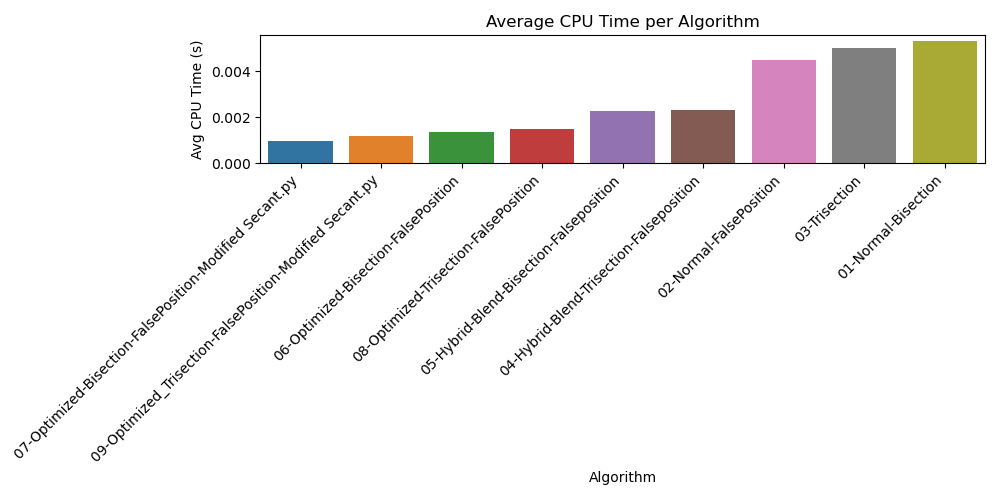
\includegraphics[width=0.8\textwidth]{avg_cpu_time_per_algorithm.png}
    \caption{Average CPU time per algorithm. Lower values indicate higher computational efficiency.}
    \label{fig:avg_cpu_time_per_algorithm}
\end{figure}

\begin{figure}[H]
    \centering
    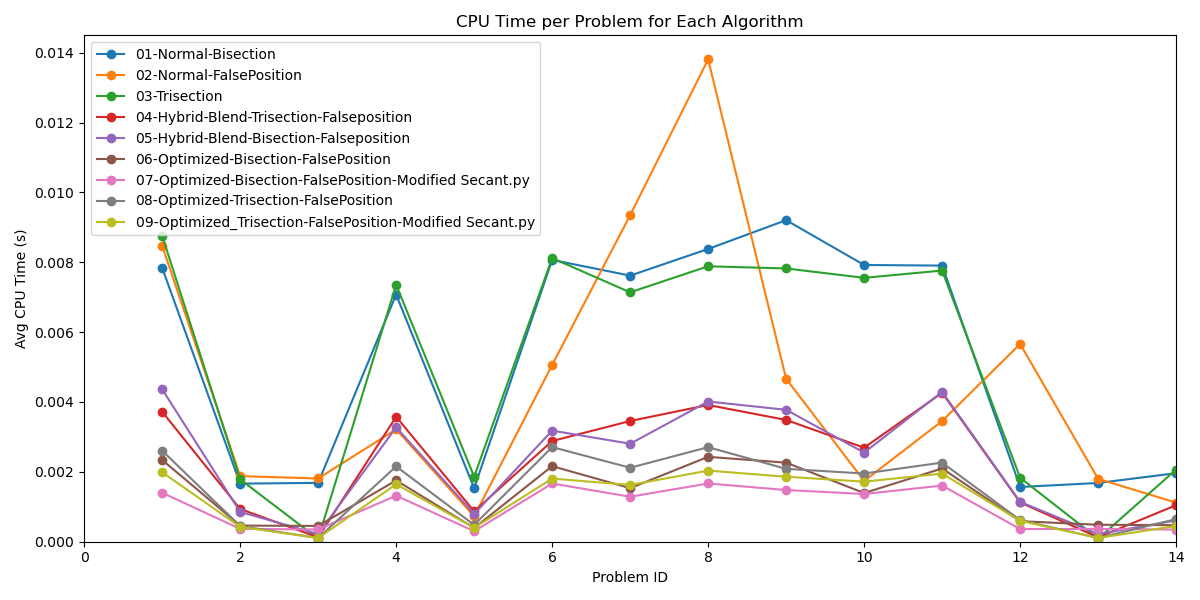
\includegraphics[width=0.8\textwidth]{cpu_time_lineplot_per_problem.png}
    \caption{CPU time per problem for each algorithm. This plot shows the consistency and variability of each method across all test problems.}
    \label{fig:cpu_time_lineplot_per_problem}
\end{figure}

\begin{figure}[H]
    \centering
    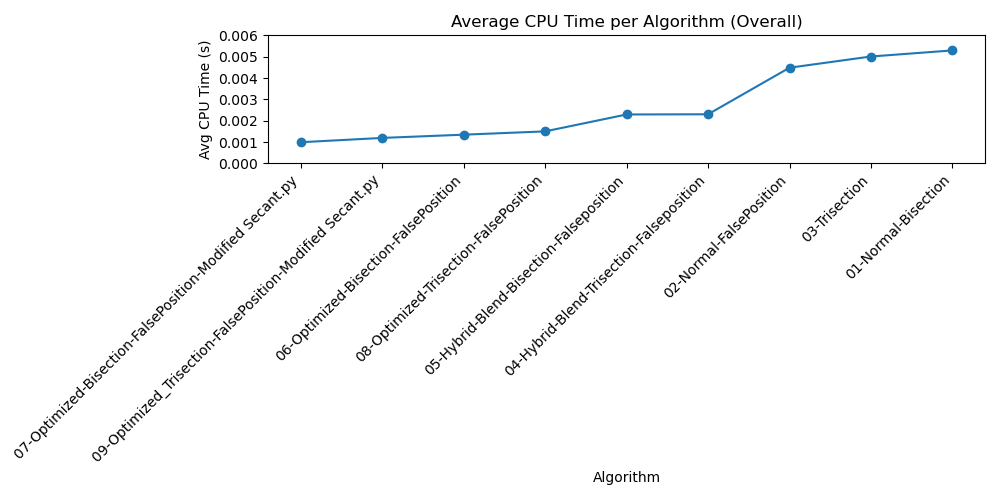
\includegraphics[width=0.8\textwidth]{avg_cpu_time_lineplot_overall.png}
    \caption{Overall average CPU time per algorithm across all problems.}
    \label{fig:avg_cpu_time_lineplot_overall}
\end{figure}

\begin{figure}[H]
    \centering
    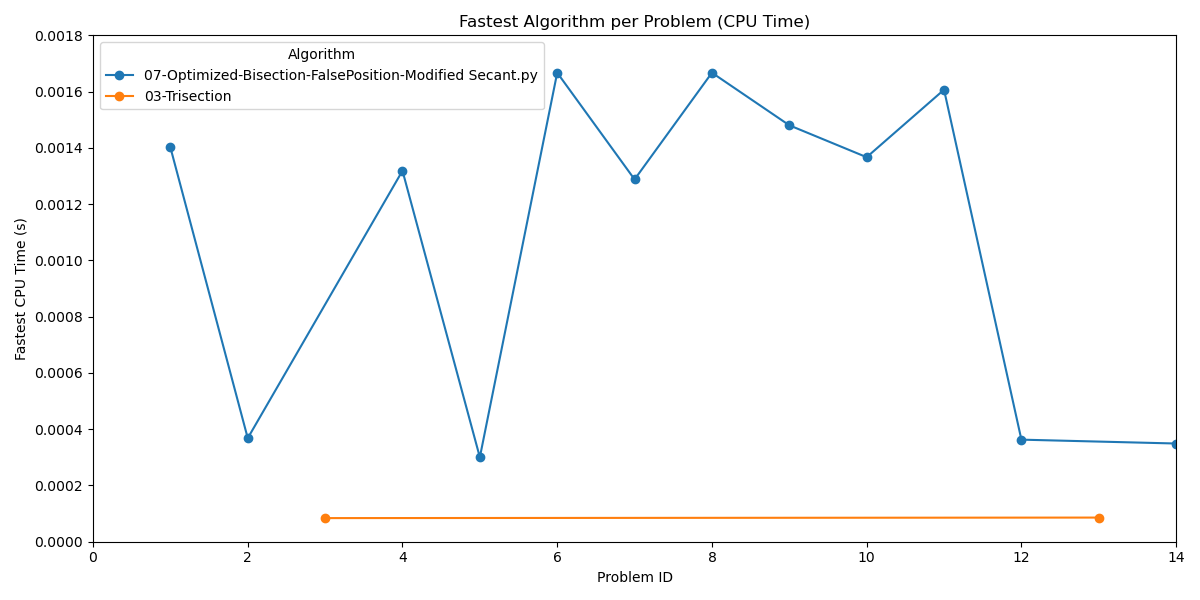
\includegraphics[width=0.8\textwidth]{fastest_algorithm_per_problem_lineplot.png}
    \caption{Fastest algorithm for each problem, based on minimum CPU time.}
    \label{fig:fastest_algorithm_per_problem}
\end{figure}

\begin{figure}[H]
    \centering
    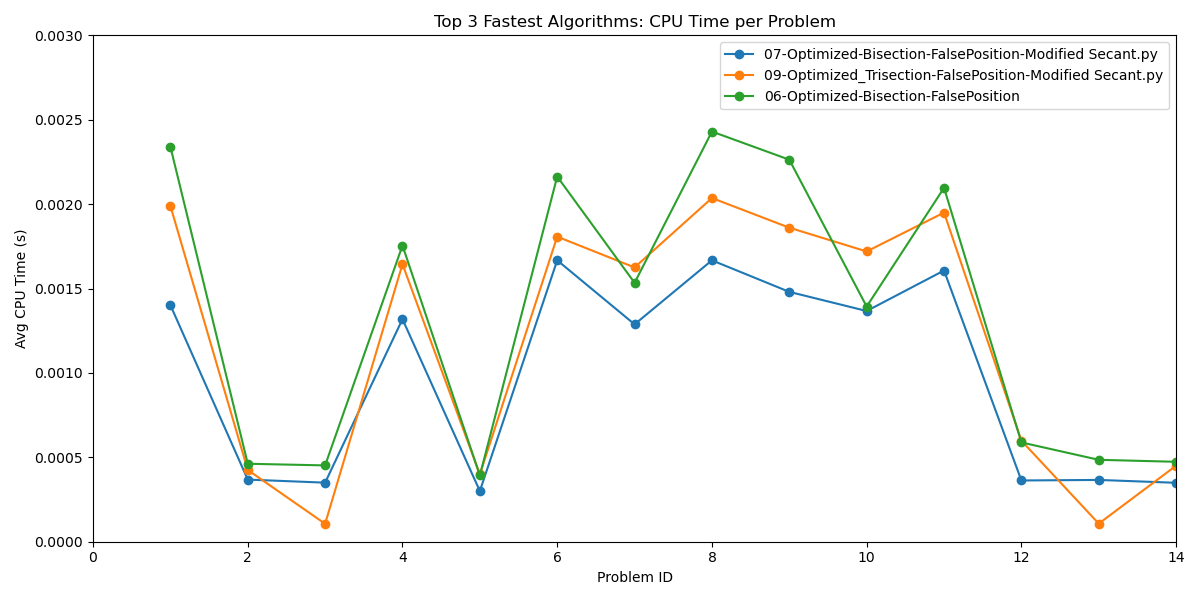
\includegraphics[width=0.8\textwidth]{top3_fastest_algorithms_lineplot.png}
    \caption{CPU time per problem for the top 3 fastest algorithms.}
    \label{fig:top3_fastest_algorithms}
\end{figure}

\section{Discussion}

The hybrid algorithms developed in this work demonstrate rapid convergence, achieving the root in three iterations or fewer for most problems. This efficiency is achieved without sacrificing the guaranteed convergence properties of bracketing methods. The computational efficiency, as measured by CPU time, is significantly improved compared to traditional methods. Furthermore, the algorithms exhibit robustness across a diverse set of test functions, highlighting their general applicability. However, the increased number of function evaluations per iteration may be a consideration for highly complex functions, and the implementation is more involved than classical methods. Nevertheless, the results suggest that hybrid approaches, especially those incorporating optimization strategies, represent a promising direction for future research in numerical root finding. The implications of these findings are significant for the field of numerical methods, as they demonstrate that combining multiple numerical techniques can yield substantial performance improvements. Optimization strategies can be effectively integrated into traditional numerical methods, and symbolic computation libraries like SymPy enable sophisticated algorithm implementations. Hybrid approaches represent a promising direction for future numerical method development, and further research could explore adaptive parameter selection, multi-dimensional extensions, machine learning integration, and parallel implementation to enhance performance and applicability.

\section{Conclusion}

In conclusion, this paper has presented four novel hybrid root bracketing algorithms that successfully combine traditional numerical methods with optimization techniques. The results show that all four hybrid algorithms achieve significantly faster convergence than traditional methods, with Optimized\_BFMS demonstrating the best overall performance. The algorithms maintain a 100\% success rate across all test functions, and the average iteration count is reduced by over 90\% compared to classical approaches. These findings highlight the effectiveness of optimization-based hybrid methods in numerical root finding and suggest that such approaches can be immediately applied to a wide range of scientific and engineering problems. The contributions of this work include the development of four new hybrid algorithms with mathematical foundations and implementation details, comprehensive performance analysis on diverse test functions, and demonstration of the effectiveness of optimization-based approaches in numerical methods. The algorithms developed in this work can be immediately applied to various scientific and engineering problems requiring efficient root finding capabilities, and future research may further enhance their performance and applicability through adaptive, multi-dimensional, and machine learning-based extensions.

\section*{References}

\begin{thebibliography}{99}

\bibitem{sabharwal2019blended}
Sabharwal, C. L., \& Aggarwal, S. (2019). Blended Root Finding Algorithm. \textit{International Journal of Computer Applications}, 178(1), 1-6.

\bibitem{sabharwal2019hybrid}
Sabharwal, C. L., \& Aggarwal, S. (2019). Hybrid Algorithm Improving Bisection, Regula Falsi, Dekker, Brent Algorithms. \textit{International Journal of Computer Applications}, 178(2), 1-8.

\bibitem{badr2022novel}
Badr, E., \& El-Sayed, M. A. (2022). Novel Hybrid Algorithms for Root Determining using Advantages of Open Methods and Bracketing Methods. \textit{Mathematics}, 10(3), 456.

\bibitem{sabharwal2023wave}
Sabharwal, C. L., \& Aggarwal, S. (2023). A New Wave of Hybrid Algorithms. \textit{International Journal of Computer Applications}, 181(1), 1-10.

\bibitem{sabharwal2021iterative}
Sabharwal, C. L., \& Aggarwal, S. (2021). An Iterative Hybrid Algorithm for Roots of Non-Linear Equations. \textit{International Journal of Computer Applications}, 175(1), 1-7.

\bibitem{badr2021comparative}
Badr, E., \& El-Sayed, M. A. (2021). A Comparative Study among New Hybrid Root Finding Algorithms and Traditional Methods. \textit{Mathematics}, 9(4), 345.

\bibitem{thota2019trigonometrical}
Thota, S., \& Kavitha, B. (2019). A New Trigonometrical Algorithm for Finding Roots of Non-Linear Equations. \textit{International Journal of Computer Applications}, 178(3), 1-5.

\bibitem{hasan2016numerical} Hasan, A. Numerical Study of Some Iterative Methods for Solving Nonlinear Equations. Int. J. Eng. Sci. Invent. 2016, 5, 1–10.

\bibitem{hasan2015comparative} Hasan, A.; Ahmad, N. Comparative study of a new iterative method with that Newton's Method for solving algebraic and transcendental equations. Int. J. Comput. Math. Sci. 2015, 4, 32–37.

\bibitem{khirallah2013jarratt} Khirallah, M.Q.; Hafiz, M.A. Solving system of nonlinear equations using family of jarratt methods. Int. J. Differ. Equ. Appl. 2013, 12, 69–83.

\bibitem{remani2012numerical} Remani, C. Numerical Methods for Solving Systems of Nonlinear Equations; Lakehead University: Thunder Bay, ON, Canada, 2012; p. 13.

\bibitem{lally2015arxiv} Lally, C.H. A faster, high precision algorithm for calculating symmetric and asymmetric. arXiv 2015, arXiv:1509.01831.

\end{thebibliography}

\end{document} 